\section{Problem definition} % (fold)
\label{sec:problem_definition}
We phrase the problem to solve as follows:

\begin{quote}
Consider an intrinsic complex system with observable dynamics and a measurable performance metric. Let this intrinsic system attains a performance metric value $X$. Introduce agents into the system with designed specific behaviors, getting an augmented system. Can we design such behaviors so that the performance metric of the augmented system attains an new value $Y$, corresponding to a better or specific behavior?
\end{quote}

We will refer at that question as the \textbf{Intrinsic System Augmentation Problem} (ISAP). We believe that this formulation accurately describe an engineering methodology for different applications. Moreover, we argue that it is easy to represent different problems with that framework.

The problem is decomposed in its most abstract formulation in Section~\ref{sec:decomposition}. But for this project and thus the rest of this report, we only look at a specific instance of it. Referring to the vocabulary and decomposition of Figure~\ref{fig:general_decomposition}, we have:
\begin{enumerate}
	\item An intrinsic complex system representing an assembly task of a puzzle (Section~\ref{sec:definition_of_the_puzzle_test_case}). This assembly task is either a self-assembly process or an assembly process depending on the components we put in and how we look at it. This intrinsic complex system is created on a simulated robotic platform (Section~\ref{sec:webots_implementation}).
	\item A mathematical model based on a Chemical Reaction Networks formulation (Chapter~\ref{cha:mathematical_model_of_the_puzzle_test_case}). We chose this formulation for its versatility and power, and because it is a well studied model with efficient simulations and theoretical insights.
	\item An control/optimization of the model using a Convergence time optimization scheme, following the work done on Rapid Mixing Markov Chains for redistribution of a swarm of robots on multiple sites~\cite{ref:BermanTRO08}. This performs a continuous optimization of our Chemical Reaction Network, namely its reaction rates. We do not address directly in this work the discrete optimal design of this Chemical Reaction Network. See Chapter~\ref{cha:chemical_reaction_networks_control_and_design}.
	\item An augmented system presented in two different ways: either modifying the behavior of the available agents or introducing new agents with designed behaviors. These are two aspects of the same augmentation process, which have different applicability fields and intrinsic difficulties. See Chapter~\ref{cha:augmented_assembly_implementation}.
\end{enumerate}

% section problem_definition (end)

\section{Decomposition} % (fold)
\label{sec:decomposition}

Starting from the definition of the ISAP, we derive a very abstract decomposition into smaller scale components. See Figure~\ref{fig:general_decomposition} for the general decomposition of the problem. See Section~\ref{sub:project_components} for a precise definition of each elements.

\begin{figure}[ht!]
	\centering
		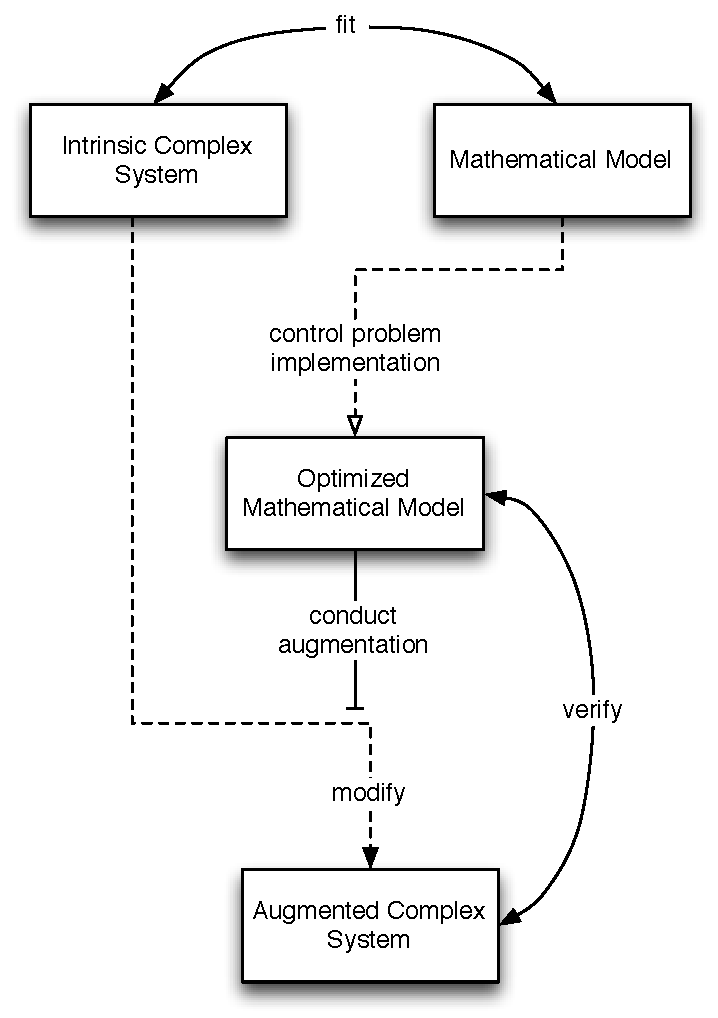
\includegraphics[width=8cm]{img/general_decomposition.pdf}
	\caption{Intrinsic System Augmentation Problem decomposition, top-level components only.}
	\label{fig:general_decomposition}
\end{figure}

Here is the rationale behind this decomposition:
\begin{enumerate}
	\item We have an Intrinsic Complex System that we are able to measure in some way. We will actually present a different formulation of this Intrinsic Complex System, for cases where the real system is not easily measurable, the Compliant Platform. We need to have some insight on this Intrinsic Complex System, because we want to model it mathematically.
	\item We construct and fit a Mathematical Model of this Intrinsic Complex System. We can use this Mathematical Model to predict the Intrinsic Complex System, and will do several iterations to get the best model possible. Different modeling approaches can be taken, as well as simulations strategies for each of them.
	\item We take this Mathematical Model and express it as a control problem to be solved. The goal can be to optimize the model for a given metric, or to change its behavior towards a specific one. This can take a lot of forms, depending on the modeling framework used and the level of plasticity available in the model and initial system. This new model can also be simulated, to verify its behavior.
	\item This Augmented Mathematical Model is used to direct the augmentation of the Intrinsic Complex System into an Augmented Complex System. By ``augmented'', we mean modifying the system global behavior using one of some of the following ideas: adding new components, modifying behaviors, modifying components. This is a Top-down approach to complex system control. Once we know how to augment the intrinsic system, we have to verify that it indeed behaves like the optimized model. Hence we perform several iterations of the augmentation, so that the optimized mathematical model actually captures the new Augmented Complex System.
	\item We can then study the Augmented Complex System, to see what was changed for it to behave accordingly to our goals. This could give insights for processes that are hard to study, especially when taking the Compliant Platform approach.
\end{enumerate}

% subsection general_decomposition (end)

\subsection{Project components} % (fold)
\label{sub:project_components}

\subsubsection{Intrinsic Complex System} % (fold)
\label{ssub:intrinsic_complex_system}

See Figure~\ref{fig:img_intrinsic_complex_system} for the diagram. This component represent the actual system we want to study and modify.

There are two possibilities for this component:


\begin{figure}[h!]
	\centering
		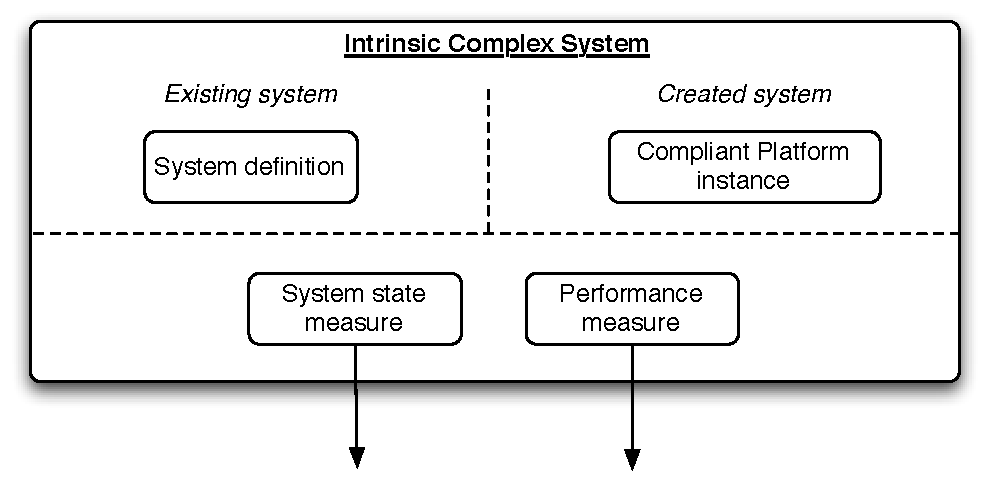
\includegraphics[width=9cm]{img/intrinsic_complex_system.pdf}
	\caption{Intrinsic Complex System component. Black arrows show inter-component communication, with other top-level components. Compliant Platform Instance in bold is defined in another diagram.}
	\label{fig:img_intrinsic_complex_system}
\end{figure}

\begin{description}
	\item[Existing system:] In that case, we have a complex system already existing. Such applications could be existing platforms for self-assembly, or an existing natural process. We need to be able to measure the state of this system in some way, as well as assessing its performance according to a desired metric. These informations are then used by the Mathematical Model component or to assess the performance of the system.
	\item[Created system:] If we do not have a complex system to observe, or if the actual complex system is not measurable, we can bypass that by \textbf{creating} an intrinsic complex system. For that we introduce a \textbf{Compliant Platform instance}. A Compliant Platform is a real or simulated platform allowing a big variety of problems reproduction. The aim is to propose a set of agents that can reproduce any given problem compatible with their hardware capabilities. Moreover, it is possible to ensure certain properties, for example a well-mixed property.
\end{description}

In this work, we use a Created system approach to reproduce a self-assembly task using a macro-scale robotic platform. The system is created using a physical simulator, Webots. More on that is presented in Chapter~\ref{cha:puzzle_test_case_implementation}.

% subsubsection intrinsic_complex_system (end)

\subsubsection{Mathematical model} % (fold)
\label{ssub:mathematical_model}

The Mathematical model component aims at reproducing as well as possible the Intrinsic Complex System, while being quicker to simulate. See Figure~\ref{fig:img_mathematical_model} for the diagram of this component.

\begin{figure}[h!]
	\centering
		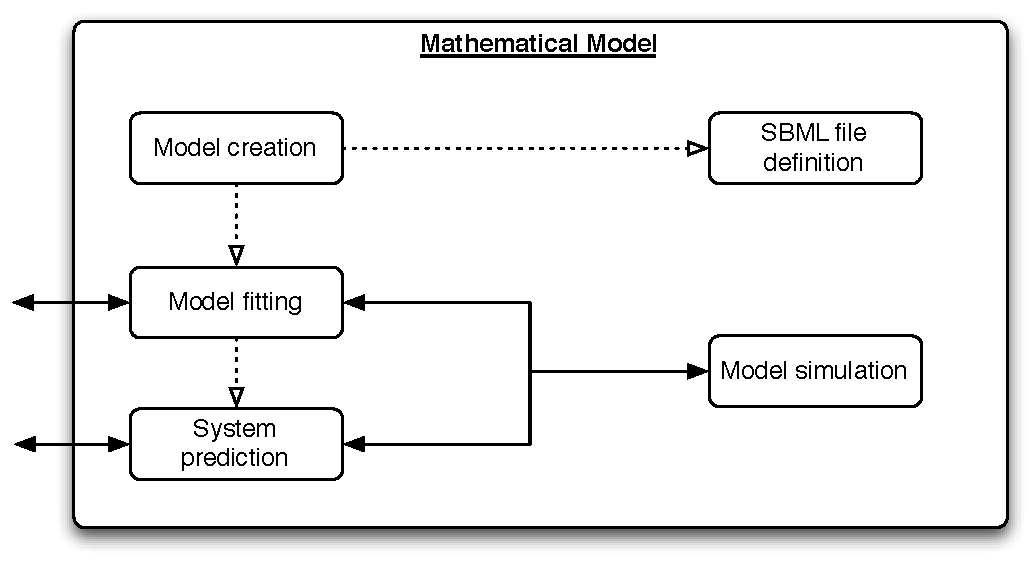
\includegraphics[width=9cm]{img/mathematical_model.pdf}
	\caption{Mathematical Model component. Black arrows show inter-component communication. Dotted arrows show termination dependencies between components.}
	\label{fig:img_mathematical_model}
\end{figure}

\begin{my_itemize}
	\item The first step is to create the model. This creation consists on the choice of a modeling notation and depends on the knowledge we have about the system. As precised earlier, we are working with Chemical Reaction Networks, so our models will be done in this framework.
	A convenient and standardized format for such networks exists: System Biology Markup Language (\textbf{SBML})~\cite{Hucka:2003p7447}. This is a XML-based file format designed to store systems of chemical reactions. This is the closest to an accepted standard we found to write our mathematical models.
	\item The model has to be fitted in some way to the Intrinsic Complex System. If we are using an existing complex system, then this is a quite complex problem, especially if we do not have precise insight in the behavior of the system. We can use methods like Bayesian Inference or MCMC (Markov Chain Monte Carlo) to fit the model on the experimental data. If we are using the Compliant Platform, than we assume that we can measure much more precisely the processes taken place, and this model fitting is more straightforward.
	\item We also need a simulation framework for the mathematical model. For Chemical Reaction Networks, a lot of literature is available on that. As we will present in Section~\ref{sub:simulation_algorithms}, we use either a direct Stochastic simulation or a simple ordinary differential equation solver.
\end{my_itemize}

% subsubsection mathematical_model (end)

\subsubsection{Optimized Mathematical model} % (fold)
\label{ssub:optimized_mathematical_model}

We use the mathematical model of our system as a thinking abstraction and an optimization medium. The model is easier to manipulate and adapted to common optimization and design techniques.

Moreover, we will use optimizations scheme that work ``blindly'', that is which have no insight into the system concepts. We think it makes the optimization more fair. Humans tend to make bad assumptions or look only for particular patterns when trying to optimize a system, we think enforcing the ``blindness'' in the algorithm could prevent that. 

Our models are multi-affine systems of equations, which are not trivial systems to analyze and optimize. We will address this issue and how we tackled it in Chapter~\ref{cha:chemical_reaction_networks_control_and_design}.

See Figure~\ref{fig:img_controlled_mathematical_model} for this component's diagram. 

\begin{figure}[h!]
	\centering
		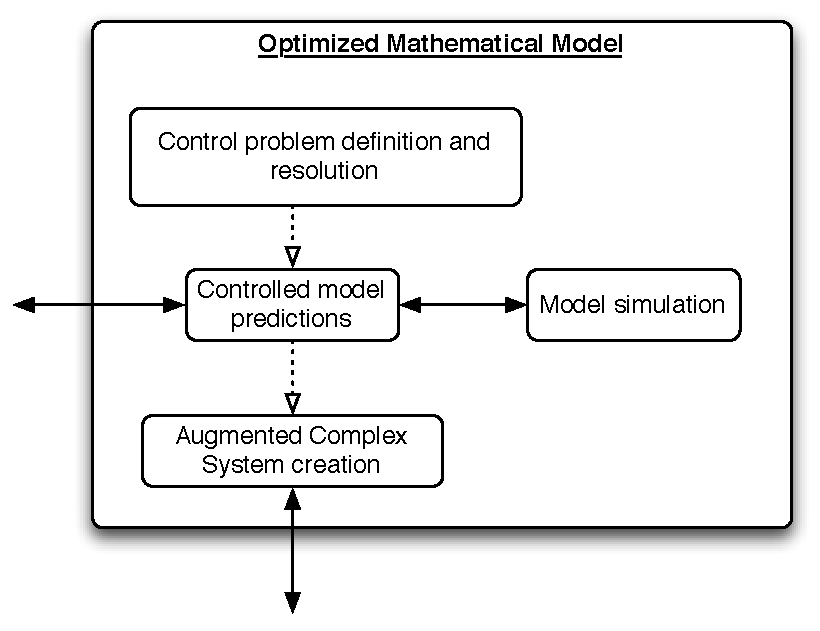
\includegraphics[width=9cm]{img/controlled_mathematical_model.pdf}
	\caption{Augmented Mathematical model component. Black arrows show inter-component communication. Dotted arrows show termination dependencies between components.}
	\label{fig:img_controlled_mathematical_model}
\end{figure}
		
% subsubsection optimized_mathematical_model (end)

\subsubsection{Augmented Complex System} % (fold)
\label{ssub:augmented_complex_system}


We then need to map the new mathematical model onto the complex system, a step we call system augmentation. This is a Top-down optimization approach, which we think is more appropriate for the kind of complex systems we are handling. This makes even more sense if we do not know a-priori how to change the behavior of the intrinsic complex system, because of its complexity. Working on the model gives another level of abstraction that helps to understand the acting processes of the complex system.

Identifying what has to be changed to produce the behavior of the modified model is a great challenge. As we will see in Section~\ref{sec:results_and_limitations}, our test case is actually very easy to modify.

See Figure~\ref{fig:img_augmented_complex_system} for the component's diagram.

\begin{figure}[h!]
	\centering
		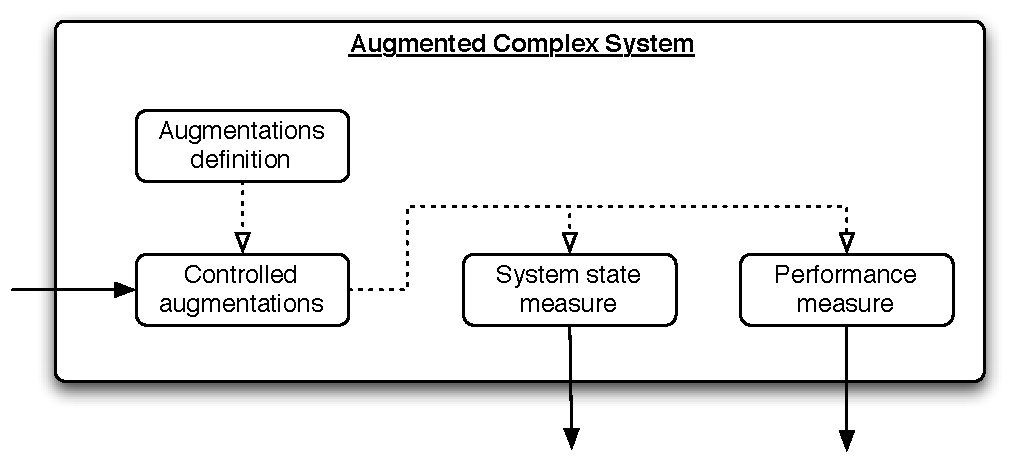
\includegraphics[width=9cm]{img/augmented_complex_system.pdf}
	\caption{Augmented Complex System model component. Black arrows show inter-component communication. Dotted arrows show termination dependencies between components.}
	\label{fig:img_augmented_complex_system}
\end{figure}

% subsubsection augmented_complex_system (end)
% subsection project_components (end)

% section decomposition (end)

\section{Examples} % (fold)
\label{sec:examples}

We quickly present some examples of several systems into our Intrinsic System Augmentation Problem framework.

\subsection{Nanoscale self-assembly} % (fold)
\label{sub:nanoscale_self_assembly}
The intrinsic system consists of the possible interactions and bonds. The augmented system can be abstracted as any modification applied to the system, that modify the intrinsic behavior. For example, changing the pH of the solution so as to activate different sticking surfaces is an action of the augmented system.
% subsection nanoscale_self_assembly (end)

\subsection{LEURRE project} % (fold)
\label{sub:leurre_project}
LEURRE is a project on building and controlling mixed societies composed of animals and artificial agents~\cite{Halloy:2007p10740}. A small robot capable of infiltrating a cockroach group was developed. The cockroach group is put in a arena with several shelters of specific luminosity. Cockroaches decide on a shelter according to the luminosity and the number of cockroaches under it. This is a self-organized decision process.
The robot were able to infiltrate this group and to direct the global decision of the group. The infiltrated robots made the cockroaches go under a light shelter, a configuration which was never attained with the cockroaches group only.

\begin{description}
	\item[Intrinsic system:] the cockroach group. The metric is the probability of the different shelters as final decision.
	\item[Augmented system:] the cockroaches and the robots. The robots choose a different shelter, this action in turn modify the final probability of the shelters.
\end{description}
% subsection leurre_project (end)

\subsection{Enzymes} % (fold)
\label{sub:enzymes}
In living cells, chemical reactions take place whenever compounds need to be transformed or created. For chemical processes needing energy to occur, one usually see an \textit{energy barrier} mechanism, see Figure~\ref{fig:img_enzyme_activity}. Before a reaction can occur, activation energy has to be provided, to pass the barrier. When adding enzymes to the system, they catalyze the reaction and produce a virtual decrease of the needed activation energy. Enzyme can act by improving fitting of compounds, stabilizing transitions or modifying orientations.

\begin{figure}[h]
	\centering
		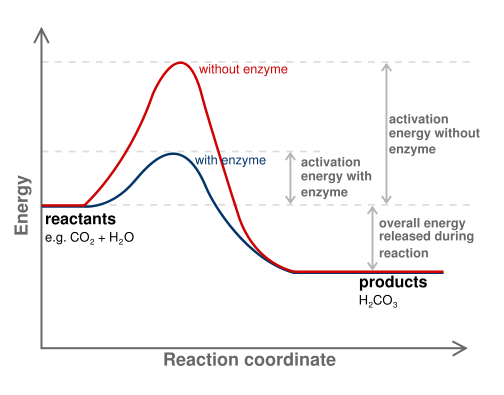
\includegraphics[width=8cm]{img/enzyme_activity.png}
	\caption{Energy barrier and catalyst effect of enzymes.}
	\label{fig:img_enzyme_activity}
\end{figure}

\begin{description}
	\item[Intrinsic system:] The original chemical reaction, with specific activation energy and rates.
	\item[Augmented system:] The catalyzed chemical reaction with the introduction of the enzyme. The enzyme performs an action (binding with change of conformation) that reduces the activation energy and increase the rate of the chemical reaction.
\end{description}

% subsection enzymes (end)

\subsection{RNA translation into proteins} % (fold)
\label{sub:protein_biosynthesis}
In living cells, DNA contains the blueprints for every functional proteins. In the cell nucleus, it is first transcripted into RNA, which is translocated to the cytoplasm to be translated into proteins. The RNA strands contains the building plan, and special proteins, called ribosomes, attach on it in order to ``read'' it and assemble amino acids (the basic building blocks of proteins) according to this plan. These amino acids are created as a linear chain (\textit{first} structure), that fold onto itself according to low-energy bounds, acquiring a tridimensional structure called a \textit{conformation} (\textit{second} and \textit{tertiary} structure). A protein is a sequence of amino acids in a specific conformation that allows its functional activity.

\begin{description}
	\item[Intrinsic system:] Ribosomes assemble amino acids according to the RNA code. The obtained first structure protein then folds itself into a specific conformation.
	\item[Augmented system:] Chaperone protein helps the folding of the protein, possibly modifying the obtained conformation or allowing the initial one under different environment conditions (heat-shock response).
\end{description}
% section examples (end)